\documentclass[conference]{IEEEtran}
\IEEEoverridecommandlockouts
% The preceding line is only needed to identify funding in the first footnote. If that is unneeded, please comment it out.
\usepackage{cite}
\usepackage{amsmath,amssymb,amsfonts}
\usepackage[T1]{fontenc}
\usepackage{algorithmic}
\usepackage{amsmath,amssymb,amsfonts}
\usepackage{graphicx}
\usepackage{subfig}
\usepackage{textcomp}
\usepackage{xcolor}
\usepackage{listings}
\usepackage{hyperref}
\def\BibTeX{{\rm B\kern-.05em{\sc i\kern-.025em b}\kern-.08em
    T\kern-.1667em\lower.7ex\hbox{E}\kern-.125emX}}
\begin{document}

\title{MACHINE LEARNING APPROACH FOR THE PREDICTION OF THE STATUS OF TANZANIAN WELLS [COMP4030 CW2 - Data Science and Machine Learning]
}

\author{\IEEEauthorblockN{*Thomas Cotter}
\IEEEauthorblockA{\textit{Computer Science} \\
\textit{University of Nottingham}\\
Nottingham, England\\
psytc8@nottingham.ac.uk}
\and
\IEEEauthorblockN{*Loo Yang Shen Jason}
\IEEEauthorblockA{\textit{Computer Science} \\
\textit{University of Nottingham}\\
Nottingham, England \\
hfyyl5@nottingham.ac.uk}
}

\maketitle

\begin{abstract}
  This paper details our approaches and results for the COMP4030 CW2. We have used a number of machine learning algorithms in order to predict the status ('Functional', 'Functional - Needs Repair' \& 'Non-Functional') of water wells in Tanzania. This is important as not only does knowing the status of the well help keep the total percentage of functioning wells higher, but it also allows for more effective spending from the government as they no longer would have to send workers out to check the status of the well. Our results suggested that the most important features were \textbf{ADD RESULTS}, and the best classification model as \textbf{ADD RESULTS}
\end{abstract}

\begin{IEEEkeywords}
  Machine Learning, Data Science, Classification
\end{IEEEkeywords}

\section{Introduction}

This section will provide an introduction to the dataset and the research questions we have attempted to solve.

\subsection{Research Questions}

We have decided that our research question will be: 

\textbf{What factors are most important for determining the status of a well, and how accurately can we classify wells based on these features?}. 

We choose this question because we are interested in the factors that determine the status of a well, and using ML to try to classify these wells into 1 of 3 classes: Functional, Non-Functional \& Functional Needs Repair. From this question, we can think about some follow-up questions. These could include:
    \begin{itemize}
        \item How does the accuracy of the classification model vary with different feature sets and classification algorithms?
        \item Could we use our results to ensure that wells are built and repaired so that fewer wells are non-functional?
    \end{itemize}

\subsection{Dataset}

We will be using the dataset from the Tanzanian Ministry of Water, which contains information on the status of wells in Tanzania to answer our research question. This dataset has 59400 rows, with 40 different features. These 40 features could be broken down into three subgroups which hold information regarding: a) Geographic Location of the Wells. b) Management of the wells. and c) Water Condition of the wells. The dataset is originally split into 2 different files, one for labels and one for the actual data. These can be merged easily with pandas through left join on the "ID" column. 

Fig. \ref{fig:status_groups} shows the distribution of the target variable, which is the status of the well. We can see from this that we might need to oversample the 'functional needs repair' class.

\begin{figure}[h]
    \centering
    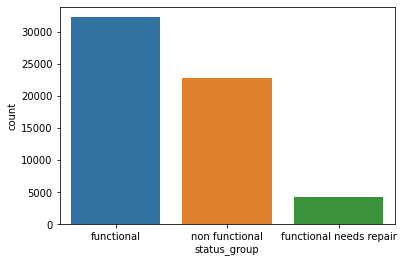
\includegraphics[scale=0.5]{figures/status_groups.png}
    \caption{Distribution of the target variable}
    \label{fig:status_groups}
\end{figure}

\subsection{Management Structure}

\textbf{Talk about the christmas tree structure of our approach to solving this problem.}

\textbf{Talk about Author Name comments}

\section{Literature Review}

In this section, we review the relevant literature on predicting machine failure, with a focus on studies that have used similar datasets to Pump It Up. Prediciting machine failure is an important area of reasearch, as it has the potential to reduce downtime and maintenance costs. Some machines may be part of a critical infrastructure, so preventing them from failure is of upmost importance.

One study by Pathak et al. (2023) \cite{pathak2023pump} compared the performance of TabNet, a sequential attentive classification architecutre designed for tabular data, and tree-based approaches such as XBBoost. They found that TabNet outpeformed XGBoost, boasting an 83\% accuracy compared to XGBoosts 78\%. TabNet makes use of Transformers, a machine learning algorithm which uses self-attention to differentially weight the significance of each part of the input. A point of note is that TabNet does not require feature engineering to perform at these standards. While TabNet is an interesting solution, we have not used it in our report, as our primary goal was to showcase an end-to-end machine learning solution, and this includes feature enginering.

Jabeur et al \cite{JABEUR2021} conducted a detailed review of different algorithms for predicting financial distress, including, SVMs, Neural Networks, RandomForest, XGBoost \& CatBoost. They found that the ensemble methods worked the most effectively (RandomForest, XGBoost \& CatBoost). Ensemble methods combine multiple models in order to improve accuracy. 

Similary, Mahabub \cite{Mahabub2020} investigated the effectiveness of ensemble methods to detect fake news. They found that combining different classification methods into a Ensemble Voting Classifier produced the best results.

Finally, Celikmih et al \cite{celikmih2020} used classification models to predict the failure of aircraft equipment and employed the ReliefF feature selection algorithm. This algorithm estimates feature weights iteratively, according to their ability to make a distinction between neighboring models. They used this to select the best subset of features to feed into their classification model, resulting in the best performance.

\section{Methodology}

\subsection{Data Analysis}

When conducting data analysis, the python library Seaborn \cite{seaborn} was our primary data visualization tool. We found that Seaborn produces more visually appealing graphs than those produced by MatPlotLib and the library itself is simpler to use. We used this alongside Pandas \cite{pandas}, a python library for advanced data handling. The results obtained from our initial data analysis guided our pre-processing decisions. (See \ref{ref:results} for detailed results).

\subsubsection{Thomas}

Thomas produced visualizations of the waterpoint \& management type distributions for each decade as well as a line chart plotting count against construction-year. The objective behind these graphs was to determine the possibility of using other values in the dataset to fill in the missing construction year data. This be discussed further in \ref{ref:results}

\subsubsection{Jason}

Jason checked the number of missing and unique values across 38 features provided. The main reasoning behind it was to identify features that would require imputations due to missing or invalid values. In addition, this step allowed him to distinguish features which would have to be recategorised due to the large number of unique values present.  He also generated Count Plots for each of the previously mentioned features based on water wells' status. These plots allowed him to visualise the distribution of the wells' status based on features. Thus, making it easier to identify features that could possibly influence the status of a water well.

\subsection{Data Preprocessing}

During the pre-processing phase, we followed our Christmas tree planning approach, working separately before combining our respective results. We each tried different techniques for pre-processing to determine the optimal ones. We both used pandas techniques to format the data in the format we wanted. Pandas is fast data manipulation tool, which makes it perfect for this problem. In this phase, we also implemented feature engineering and data cleaning approaches.

\subsubsection{Thomas}

Thomas initially performed the imputation of the latitude \& longitude missing values by applying mean imputation with a specific approach. Firstly, the data was grouped by 'ward', followed by calculating the mean for the missing lat/lon values. If any NaNs remained (e.g. due to missing 'ward' information), then the data was grouped by 'LGA' and the process repeated. Finally, the data was grouped by 'region', ensuring no missing values were left. The will be discussed further in \ref{ref:results}.

He also looked at the Funder \& Installer columns, which contained 1000s of unique values. In his approach, he decided to group the column into Seven categories: 'Charity', 'Government', 'Local Government', 'Private', 'Religious', 'Foreign' \& 'School'. This was done to simplify the dataset, making it easier for the model to learn the distribution. Finally, Thomas also used the SMOTE-ENN algorithm from imblearn \cite{smote-enn}, to balanced the imbalance in the 'Functional - Needs Repair' class. Imbalanced datasets could potentially affect model performance, especially in tree-based models.

\subsubsection{Jason}

Due to the presence of missing data in the Latitude \& Longitude columns, Jason decided to apply mean imputation based on the Region column. The values of the Region column corresponds with the name of cities present in Tanzania. By calculating the  mean latitude and longitude value of each region, a rough estimation of the geographical location of wells with missing value could be known. Therefore, allowing valuable insights to be learnt by ML models during training.

During the Data Analysis Phase, he had noticed that two columns Permit and Public Meeting had missing values. Upon further inspection, these two columns only contain the values of either 'True' or 'False'. Data Imputation was not done at this stage due to the lack of valuable data present in the data set. To preserve the distribution of these two columns, a unique values known as 'Unknown' was given to rows with missing data.

Jason had performed data recategorisation on both funder and installer columns which contained 1000 - 2000 unique values. He had first performed data cleaning to fix spelling mistakes that were present in each column. This was followed by identifying unique values with count above the threshold of 1000. Each unique value above the previously mentioned threshold would be classified as its own individual class while those below it would be classified under the 'Other' value. Data recategorisation would be able to reduce the number of unique values present in these two columns leading to better ML model training performance.

Although the number of unique values in the Region Column are minimal, Jason decided to reclassify them according to their geographical zones based on data that was provided by the Tanzania Water and Sanitation Network \cite{tawasanet}. This reduced the number of unique values of the Region Column to 7 from 21. New insights could potentially be drawn upon  based on the zone that the water wells is currently located in.

The data set provided had feature and target variables in the form of categorical form. Jason had converted these features into numerical form that is required of by ML models prior to training. He had encoded the values of the feature and target variables in the form of alphabetical order whereby a = 0, b = 1 etc. 

\subsection{Data Classification}

 To classify the data, we utilized various classification algorithms. Initially, our focus was on testing the performance of different algorithms without any feature selection. This would allows us to focus on the best performing ones. The results from this test can be seen in Table. \ref{tab:initial-clf-results}. From these results, we can see that XGBoostClassifier, CatBoostClassifier, BaggingClassifier \& HistGradientBoostingClassifier were the most effective for our problem. We decided to fully explore these models using feature selection \& hyper-parameter tuning. Our feature selection process employed a Chi-Squared test and feature importance obtained from a RandomForest to generate a subset of potential features.

\begin{table}[h]
  \centering
  \caption{Initial Classification Results}
  \label{tab:initial-clf-results}
  \begin{tabular}{|c|c|c|c|}
    \hline
    \textbf{Algorithm} & \textbf{Accuracy} & \textbf{Precision} & \textbf{Recall} \\ \hline
    XGB	& 0.797811 & 0.751084 & 0.632675 \\
    \hline
    CatBoost & 0.794865 & 0.745754 & 0.633800 \\
    \hline
    Bagging & 0.793434 & 0.704477 & 0.658841 \\
    \hline
    HistGradientBoosting & 0.790909 & 0.743381 & 0.623847 \\
    \hline
    DT & 0.756902 & 0.643165 & 0.644585 \\
    \hline
    KNN & 0.708754 & 0.623125 & 0.563458 \\
    \hline
  \end{tabular}
\end{table}


\subsubsection{Thomas}

Initially, Thomas followed on from the decision to balance the dataset. He trained the 4 top models (XGBoost, CatBoost, Bagging \& HGBoost) on the balanced dataset and compared the results to models trained on the unbalanced dataset. The results can be seen in \ref{ref:results}. Furthermore, he used Weights and Biases (WandB) \cite{wandb} to further analyse the subset of features produced by the Chi-Squared Test and RandomForest.  WandB provided an easy-to-use MLOps platform for tracking our experiments and helped us understand which features worked best for each classifier. He trained multiple classifiers on different subsets of the feature set (ranging from sizes 0.75N to N, where N is the size of the original feature set), and tracked this information in WandB. WandB allows us to quickly filter for the best performing 'runs', and find out which feature set was used in this run. He also used WandB to further analyse the results of our cross-validation hyper-parameter tuning, in much a similar process to feature selection.

\subsubsection{Jason}

From the Random Forest feature importance and Chi-Squared Test, Jason had shortlisted 16 features that influenced the classification of Tanzanian Water Wells. Prior to model training, the dataset was subjected to a 80\%:20\% train test split. This was followed by normalising the testing and training set features with z-score normalisation.

For this study, he considered three different machine learning models  (Random Forrest, XGBoost \& CatBoost). Hyperparameter tuning was conducted via GridSearchCV \cite{gridsearch} from the sklearn library. Upon completion of the hyperparameter tuning process, the most optimal parameters of each model were recorded before being passed for model training. 

To evaluate the performance of each model, Jason used three different evaluation methods. K-fold cross validation with the value of K being 5 , confusion matrix and receiver operating characteristic (ROC) curve. K-fold cross validations was used to evaluate the performance of the model on unseen data. Meanwhile, confusion matrix showcases the predictions which are labelled correctly and incorrectly by class. Although ROC Curve is usually meant for binary classification, it could still be extended to multiclass classification through pairwise comparison i.e., one class vs all other classes.   

\section{Results} \label{ref:results}

\subsection{Data Analysis}

\subsection{Data Preprocessing}

\subsection{Classification}

\section{Discussion}

\section{Conclusion}

\bibliographystyle{plain}
\bibliography{refs}

\end{document}


